\documentclass{article}

\usepackage{../preamble}
\standalonetrue

\pagestyle{fancy}
\fancyhf{}
\rhead{Section \thesection}
\lhead{PHYS 304 Lecture 09}
\rfoot{Page \thepage}


\title{PHYS 304 Lecture 09}
\author{Ashtan Mistal}
\date{!!!}

\begin{document}

\ifstandalone
\maketitle
\fi

\graphicspath{{./Lecture09/}}

\section{Review of key points from last day}

Stationary states don’t exist for free electrons ($V=0$ in all space), because purely harmonic wavefunctions can’t be normalized (the wavefunctions don’t decay to zero at plus and minus infinity).

We deferred the resolution of this “problem” to today’s lecture, but noticed other qualitative differences in the free particle solutions of the TISE, compared to all of our previous examples.  In particular, there is:

\begin{itemize}
    \item no restriction (other than $E>0$) on the allowed energy eigen values, and 
    \item for each $E>0$ there are two independent eigen functions (complex conjugates of each other), characterized by equal and opposite wavevectors $k = \pm \sqrt{\frac{2mE}{\hbar^2}}$.
\end{itemize}

If we fudge the normalization problem by considering a very large but finite extent to the universe, the expectation value of the momentum in one of these eigen functions of the TISE is equal to $\hbar k$, corresponding to a velocity $\frac{\hbar k}{m}$. This is two times the phase velocity of the harmonic wave $e^{i(k x-\omega t)}, \omega=\frac{E}{h}$ which corresponds to a fudged stationary state for free particles.

We finally noted that the most important quality of "stationary" eigen functions in bounded potentials is their orthonormal completeness property that allows one to expand some initial wavefunction, $\Psi(x, 0)$, as a sum over all eigen functions of the time independent $\mathrm{SE}$, then tacking on the harmonic time dependence of each component, trivially, to find $\Psi(x, t)$. Crucially, this property rigorously holds even for "unnormalizable" eigen functions, when the discrete sum is replaced by a continuous integral, as we will now see.

\section{Today: Gaussian Wavepackets, group velocity, particle localization.}

[Notes are handwritten. TODO: finish and add later. ]

\subsection{Useful Equations}

\begin{enumerate}
    \item $f(x)=\frac{1}{\sqrt{2 \pi}} \int_{-\infty}^{\infty} F(k) e^{i k x} d k \leftrightarrow F(k)=\frac{1}{\sqrt{2 \pi}} \int_{-\infty}^{\infty} f(x) e^{-i k x} d x$
    \item $\int_{-\infty}^{\infty} e^{\frac{-k^{2}}{4 e}} e^{-i k x} d k=\sqrt{4 \pi c} e^{-c x^{2}}$
    \item $\int_{-\infty}^{\infty} e^{-x^{2}} d x=\sqrt{\pi}$
    \item If $\mathrm{g}(\mathrm{x})=\frac{1}{\sigma \sqrt{2 \pi}} e^{-\frac{1}{2}\left(\frac{x-\mu}{\sigma}\right)^{2}}, \int_{-\infty}^{\infty} g(x) d x=1$
    \item If $\mathrm{f}(\mathrm{x})=a e^{-\frac{(x-b)^{2}}{2 c^{2}}}$, the full-width at half maximum (FWHM) of the function centred at $\mathrm{x}=\mathrm{b}$ is: $\mathrm{FWHM}=2 \sqrt{2 \ln (2)} c \approx 2.35482 c$
\end{enumerate}

If the wavefunction of a free particle at $\mathrm{t}=0$ is expanded in terms of the (unnormalizable) eigen states (with real eigen values) of the time-independent Schrodinger equation as:
$$
\Psi(x, 0)=\frac{1}{\sqrt{2 \pi}} \int_{-\infty}^{\infty} \phi(k) e^{i k x} d k
$$

then the full wavefunction is

$$
\Psi(x, t)=\frac{1}{\sqrt{2 \pi}} \int_{-\infty}^{\infty} \phi(k) e^{i\left(k x-\frac{k^{2}}{2 m} t\right)} d k
$$

\subsection{Discussion}

\begin{enumerate}
    \item Discuss the dynamics of this state. How would you describe its evolution in time, qualitatively?
    \item How long would it take for an electron with an atomic scale localization (say $\sigma=1 \mathrm{~nm}$ for simplicity) to increase its "size" by a factor of $\sqrt{2} ? \sim 17$ femtoseconds
    \item How long would it take for an electron localized to a laboratory lengthscale (say $\sigma=1 \mathrm{~m}$ for simplicity) to increase its "size" by a factor of $\sqrt{2} ? \sim 5 \mathrm{hrs}$
    \item Can you think of a classical analogy for this behaviour?
\end{enumerate}

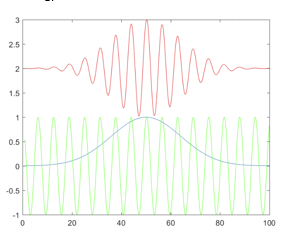
\includegraphics[width = 0.6 \textwidth]{Lecture09/image.png}

Red: net wavepacket. Blue: Envelope; $e^{- \left( (x - x_0 - \frac{\hbar k_0 t}{m})/2 \sigma \right)^2}$. Green: "carrier"; $e^{i \left( k_0 x - \frac{\hbar^2 x_0^2 t}{2m} t \right)}$

\end{document}